\documentclass[12pt,a4paper]{article}
\usepackage[utf8]{inputenc}
\usepackage[german]{babel}
\usepackage[T1]{fontenc}
\usepackage{amsmath}
\usepackage{amsfonts}
\usepackage{amssymb}
\usepackage{graphicx}
\usepackage{float}
\usepackage[left=2cm,right=2cm,top=2cm,bottom=2cm]{geometry}
\author{Tim}

\begin{document}

\tableofcontents
\newpage

\section{Kondensator}
\subsection{Versuchsbeschreibung}
In diesem Teilversuch soll die Kapazität eines Kondensators durch Auf- und Entladung von diesem bestimmt werden.
\subsubsection{Aufladung}
Wird eine Spannung an einen Kondensator angelegt, so wird dieser geladen, bis die Quellspannung kompensiert wird. Der Ladevorgang dauert umso länger, je größer der Widerstand des Stromkreises ist.\\
Aus der Maschenregel folgt:
\begin{equation}
U_0 = U_R + U_C \Rightarrow U_0 - U_C = R\cdot C\cdot \dfrac{dU_c}{dt}
\label{Kondensator_DGL}
\end{equation}
Bei der Aufladung kann man daraus den Strom und die Spannung bestimmen:
\begin{equation}
U_C(t) = U_0 \cdot (1-e^{-\dfrac{t}{R\cdot C}})
\end{equation}
\begin{equation}
I(t) = I_0 \cdot e^{-\dfrac{t}{R\cdot C}}
\end{equation}
Dabei ist $\tau = R \cdot C$ die Zeitkonstante des R-C-Kreises.
\subsubsection{Entladung}
Bei der Entladung liegt keine externe Spannung mehr an. Es gilt also: $U_0 = 0$\\
Mit dieser Annahme und Gl. \ref{Kondensator_DGL} folgt:
\begin{equation}
U_C(t) = U_0 \cdot e^{-\dfrac{t}{R\cdot C}}
\end{equation}
\begin{equation}
I(t) = -I_0 \cdot e^{-\dfrac{t}{R\cdot C}}
\end{equation}
\subsection{Aufbau und Durchführung}

\subsection{Auswertung}



\section{RLC-Schwingkreis}
\subsection{Versuchsbeschreibung}

In diesem Versuch soll die gedämpfte Schwingung eines RLC-Schwingkreises aufgezeichnet werden, sowie die Schwingungsfrequenz und Dämpfung der Schwingung bestimmt werden.
Mit diesen Werten sollen gegebenenfalls die verwendeten Bauteile charakterisiert werden.

\subsubsection{Grundlagen}
Grundlage des Versuchs ist die gedämpfte Schwingungsgleichung bei der Entladung des Kondensators

\begin{equation}
\ddot{Q}+2\delta \dot{Q}+\omega_0^2 Q=0
\end{equation}

mit der Dämpfung $\delta=\frac{R}{2L}$ und der Kreisfrequenz der ungedämpften Schwingung $\omega_0=\frac{1}{\sqrt{LC}}$.\\
Dabei müssen drei Fälle unterschieden werden:\\
Im \textbf{Kriechfall} gilt $\delta > \omega_0$. Die Spannung fällt asymptotisch gegen null ab und es findet keine Schwingung statt.\\
Der \textbf{Aperiodischer Grenzfall} liegt vor falls $\delta=\omega_0$. Der Kondensator wird in kürzester Zeit und ohne Überschwingen entladen.\\
Für $\delta<\omega_0$ liegt der \textbf{Schwingfall} vor. Die Spannungssignal ist von der Form 
\begin{equation}
U_c(t)=U_0 \cdot e^{-\delta t} \cdot \sin{\omega t} \quad \text{mit} \quad \omega=\sqrt{\omega_0^2-\delta^2}
\end{equation}
und erreicht erst nach einem Einschwingvorgang seinen Endwert.\\

Eine Charakterisierung der verwendeten Spule wird dabei über folgende Zusammenhänge ermöglicht:
\begin{equation}
L=\frac{1}{(\omega^2+\delta^2)\cdot C} \qquad  R_L=\frac{2\delta}{(\omega^2+\delta^2)\cdot C}-R_{gesteckt}
\end{equation}

\subsection{Aufbau und Durchführung}
\subsubsection{Aufbau}

Der Schwingkreis wird gemäß dem Schaltplan (Abb. \ref{fig:RLCSchaltung}) aufgebaut. Als Widerstand wurde ein Potentiometer verwendet. Der hier verwendete Kondensator hatte eine nominelle Kapazität von $C=4.7 \mu F$, für die verwendete Spule waren $R_L=9.5 \Omega$ und $L \approx 36mH$ ausgewiesen. Strom und Spannung werden mit dem CASSY gemessen. Die Einstellungen finden sich in Tab. \ref{tab:CASSY}

\begin{figure}
\begin{center}
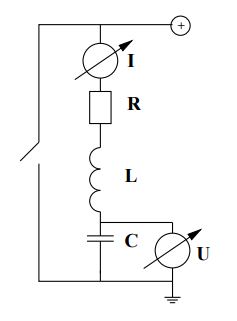
\includegraphics[scale=0.8]{Bilder/RLCSchaltung.png}
\end{center}
\caption[RLC Schaltung]{Schaltplan des RLC-Schwingkreises. (Quelle: Praktikumsskript Seite 84)}
\label{fig:RLCSchaltung}
\end{figure}

\begin{table}
\begin{center}
\begin{tabular}{|c|c|}
\hline
Messparameter &  $10 \mu s$ Messintervall;  2000 Messwerte \\
\hline
Trigger & fallend, 6V\\
\hline
Anm. & \\
\hline
\end{tabular}
\caption[CASSY]{Einstellungen CASSY}
\label{tab:CASSY}
\end{center}
\end{table}


\subsubsection{Durchführung}
Es wird die durch Entladen des Kondensators angeregte Schwingung aufgezeichnet. Dazu wird der Kondensator zunächst mit 7V Ladespannung geladen. Nach Einstellen des Widerstandes am Potentiometer (Eingesteller Wert wurde mit dem Multimeter bestimmt) wird der Schalter geschlossen. Durch den Kurzschluss der Spannungsquelle entlädt sich der Kondensator über den Widerstand. Der Verlauf der Kondensatorspannung und des Stroms werden aufgezeichnet.\\
Der Entladevorgang wurde für jede Widerstandseinstellung insgesamt fünf mal durchgeführt.


\subsection{Auswertung}
\subsubsection{Rohdaten}
Der prinzipielle Verlauf ist bei fast allen Messungen weitesgehend identisch, deswegen werden hier nur einige Spannungsverläufe exemplarisch gezeigt.

\begin{figure}
\begin{center}
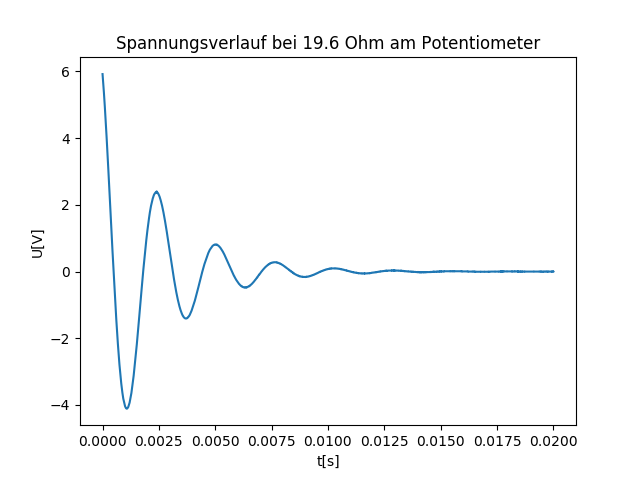
\includegraphics[scale=0.5]{Bilder/Spannungsverlauf19,6Ohm}
\end{center}
\caption[Spannungsverlauf]{Spannungsverlauf für Messung 1 bei $R=19.6 \Omega$ am Potentiometer (Multimeterangabe).}
\label{fig:Spannung19,6}
\end{figure}

...to be continued....

\subsubsection{Frequenzbestimmung}
In diesem Versuch stehen einem prinzipiell zwei Möglichkeiten zur Frequenzbestimmung zur Verfügung.
Einmal durch Fouriertransformation des gemessenen Spannungssignals und anschließender Peakbestimmung, die zweite Möglichkeit durch Bestimmung der mittleren Periodendauer des Spannungssignals.\\

Die Bestimmung mittels Fouriertransformation ist in diesem Fall nicht zufriedenstellend, da die Auflösung des Spektrums zu grob ist (siehe Abb. für das zu Abb.\ref{fig:Spannung19,6} zugehörige Frequenzspektrum).


\end{document}